\documentclass[12pt,a4paper]{article}
\usepackage[utf8]{inputenc}
\usepackage[german]{babel}
\usepackage[T1]{fontenc}
\usepackage{times}
\usepackage{graphicx}
\usepackage{url}
\usepackage{color}
\usepackage{setspace}
\usepackage{enumerate}
\usepackage{amsmath}
\usepackage{amsfonts}
\usepackage{amssymb}
\usepackage{float}
\usepackage{stix}
\usepackage{subcaption}
\usepackage{textgreek}
\usepackage{ragged2e}
\title{Zusammenfassung Informations- und Kodierungstheorie}
\author{Henrik Tscherny}
\begin{document}
\maketitle
\tableofcontents
\section{Grundlagen}

\section{Informationsquellen}
Die verschiedenen Informationsquellen können wie folgt eingeordnet werden:
\begin{itemize}
\item diskrete Quellen
\begin{itemize}
\item Einzelquellen
\begin{itemize}
\item Quellen mit unabhängigen Ereignissen
\item Quellen mit abhängigen Ereignissen (Markow-Quellen)
\end{itemize}
\item Verbundquellen
\end{itemize}
\item kontinuierliche Quellen
\end{itemize}
\newpage
\subsection{Quellen mit unabhängigen Ereignissen}

\paragraph{Entropie\\}
\begin{itemize}
\item Sei $X = \{x_1, ..., x_N \}$ das Quellenalphabet
\item Sei $p_i$ eine Menge von Auftrittswahrscheinlichkeiten mit $\sum_i^n p(x_i) = 1$
\end{itemize}
\textbf{Entropie für das Zeichen $x_i$:} $H_i = ld(\frac{1}{p(x_i)}) = -ld(p(x_i))$\\
\textbf{Quellenentropie:} $H_m = \sum_i^N p(x_i)\; H_i = -\sum_i^N p(x_i) ld(p(x_i))$\\
\textbf{Sonderfall für Gleichverteilung der Zeichen:} $H_0 = ld(N)$ gdw. $p(x_i) = \frac{1}{N}$

\subsection{Quellen mit abhängigen Ereignissen (Markow-Quellen)}
\begin{itemize}
\item Ein Ereignis tritt immer unter einer (Kette von) Vorbedingung ein (außer das erste Ereignis)
\item Die Auswahl des nächsten Ereignisses erfolgt nach einer bedingten Wahrscheinlichkeit abhängig von den Ereignissen zuvor
\item $p(x^{(m+1)}\vert x^{m}\cdots x^{(2)}\hspace{5pt}x^{(1)})$ Wahrscheinlichkeit von Ereignis (m+1) wenn Kette aus Ereignissen (m...1) eingetreten sind
\item Eine Markow-Quelle erster Ordnung berücksichtigt nur das letzte Ereignis
\begin{itemize}
\item $p(x^{(m+1)}\vert x^{(x)})$ mit $p(x_j\vert x_i)$ (Wahrscheinlichkeit von $x_j$ wenn $x_i$)
\end{itemize}
\end{itemize}

\begin{figure}[h]
\begin{subfigure}{0.5\textwidth}
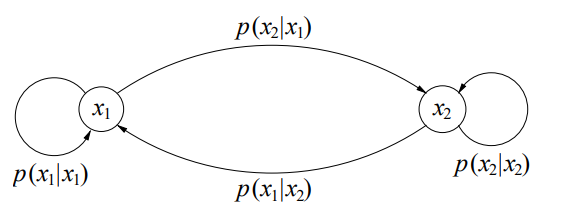
\includegraphics[scale=0.5]{resources/markow_graph.png}
\end{subfigure}
\begin{subfigure}{0.5\textwidth}
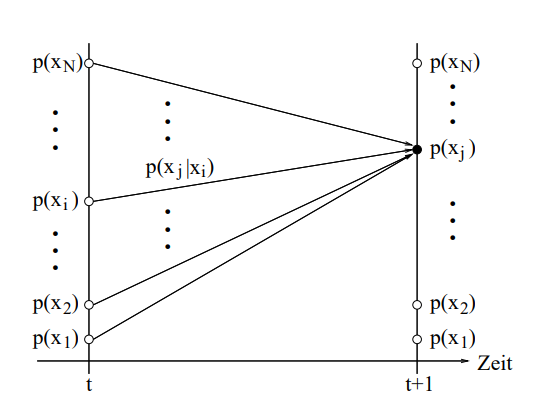
\includegraphics[scale=0.5]{resources/markow_diag.png}
\end{subfigure}
\end{figure}

\paragraph{Entropie\\}
\begin{itemize}
\item \textbf{Entropie für ein Zeichen:} $H_i = \sum_j^N p(x_j \vert x_i)\; ld(\frac{1}{p(x_j) \vert x_i)})$
\item \textbf{Markow-Entropie:} $H_M = \sum_i^N \sum_j^N \overline{p(x_i)}\; p(x_j\vert x_i)\; ld(\frac{1}{p(x_j\vert x_i)} $
\end{itemize}

\subsection{Verbundquellen}
\begin{itemize}
\item Seien X und Y diskrete Quellen
\item Sei $(p(x_i))$ und $(p(y_j)$ die zugehörigen Auftrittswahrscheinlichkeiten
\item Die Ereignisse in X und Y separat sind \textbf{unabhängig} voneinander
\item Ein Ereignis in X hat ein \textbf{bedingtes Ereignis} in Y ($p(y_j\vert x_i)$) zur Folge
\item Das Auftreten zweier Ereignisse $x_i$ und $y_j$ heißt \textbf{Verbundereignis} $(x_i, y_j)$
\item Die Wahrscheinlichkeit, dass $x_i$ und $x_j$ eintreten heißt\\
\textbf{Verbundwahrscheinlichkeit} $p(x_i,y_j) = p(x_i) \cdot p(y_j\vert x_i)$ (Satz von Bayes)
\end{itemize}
\begin{figure}[H]
\centering
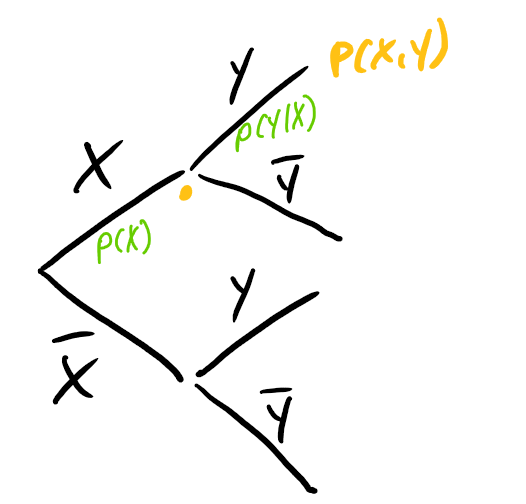
\includegraphics[scale=0.3]{./resources/verb_baum.png}
\end{figure}
Note: $p(x_i, y_j) = p(x_i\cap y_j)$


\paragraph{Entropie\\}
\begin{itemize}
\item Sei Seien X und Y diskrete Quellen mit $p(x_i,y_j)$ $\rightarrow$ \textbf{Verbundquelle (X,Y)}
\item \textbf{Verbundentropie:} $H(X,Y) = \sum_i^N \sum_j^M \; p(x_i,y_j) \; ld(\frac{1}{p(x_i,y_j)})$\\
= $H(X,Y) = H(X) + \sum_i^N \sum_j^M \; p(x_i)\; p(y_j\vert x_i) \; ld(\frac{1}{p(x_i,y_j)})$
\item \textbf{Sonderfall X,Y unabhängig:} $H(Y\vert X) = H(Y)$ und $H(X,Y) = H(X) + H(Y)$
\item \textbf{Sonderfall vollständig abhängig:} $H(Y\vert  X) = 0$ und $H(X,Y) = H(X)$
\item \textbf{Sonderfall identische Ereignismengen:} $H_M = H(X,X) - H(X)$ und $H(X) \leq H(X,X) \leq 2H(X)$
\end{itemize}

\section{Kodierung}
\paragraph{Kodwortlänge\\}
\begin{itemize}
\item \textbf{gleichmäßiger Kode}: $l = \lceil ld N \rceil$
\item \textbf{ungleichmäßiger Kode}: $l_m = \sum_i^N \; p(x_i) l_i$
\item \textbf{optimaler Kode}: Sein $q, d_{min}, n \in \mathbb{N}$, mit n... Länge, q-närer Zeichenvorrat $d_{min}$... Mindestdistanz. Es gibt keinen Kode welcher unter diesen Parameter mehr Wörter kodiert
\end{itemize}

\paragraph{Dekodierbarkeit\\}
\begin{itemize}
\item \textit{Hinreichend}: Das Ende eines Kodewortes darf nicht gleich dem Anfang eines anderen Kodewortes sein (\textbf{Präfixfrei})
\item \textit{Notwendig}: $\sum_i^N \; 2^{-l_i} \leq 1$ ($l_i$ = Kodewortlänge)\\
Auftrittswahrscheinlichkeiten der Kodewörter sind nur Zweierpotenzen
\item $l_m \geq H_m$
\end{itemize}

\paragraph{Redundanz\\}
\begin{itemize}
\item \textbf{redundanzarm}: $H_m \leq l_m < H_m + 1$
\item \textbf{redundanzfrei}: $l_m = H_m$
\item \textbf{Koderedundanz}: $R_K = l_m (\cdot H_K) - H_Q \geq 0$ ($H_K$ meist 1 $\rightarrow$ fällt weg)
\item \textbf{Mittlere Kodewortlänge $l_m$} Wahrscheinlichkeit des Zeichens * dessen Länge dessen Kodewortes
\end{itemize}

\subsection{Shannonsche Kodierungstheoreme}
\subsubsection{1. Theorem}
\begin{itemize}
\item Es ist eine redundanzfreie Kodierung auch für Auftrittswahrscheinlichkeiten welche keine Zweierpotenz sind möglich\\
$p(x_i) \neq 2^{-l_i}$
\item \textbf{Lösung:} m-Fache Erweiterung der Quelle\\
$\rightarrow$ Kodieren der Quellzeichen als Blöcke von m Zeichen
\item bildet Grundlage für die \textbf{Entropiekodierung}
\end{itemize}
\subsubsection{2. Theorem}
\begin{itemize}
\item Die \textbf{Restfehlerwahrscheinlichkeit} $p_R$ kann beliebig klein gehalten werden
\item Dazu muss aber die Koderate $R$ den Wert der Maximalen Transinformation $H_T$ nicht überschreiten
\end{itemize}

\subsection{Verfahren}
\subsubsection{Shannon-Fano-Verfahren}
\begin{enumerate}
\item Ordne Zeichen abfallend nach ihrer Auftrittswahrscheinlichkeit
\item Teile nun in zwei Teilmengen mit möglichst gleicher Wahrscheinlichkeitssumme
\item Weise den entstandenen Gruppen 1 (bzw. 0) zu (Reihenfolge egal)
\item GOTO 1 until Teilmengen nicht mehr teilbar
\end{enumerate}

\subsubsection{Huffman-Verfahren}
\begin{enumerate}
\item Ordne Zeichen abfallend nach ihrer Auftrittswahrscheinlichkeit
\item Fasse Zeichen(menge) mit der kleinsten Auftrittswahrscheinlichkeit(-Summe) zusammen
\item Ordne neu erhaltene Zeichenmengen nach ihren Auftrittswahrscheinlichkeiten
\item GOTO 2 while SUM $\neq$ 1
\item weise den entstandenen Ästen des Baumes 1 (bzw. 0) zu
\end{enumerate}

\subsection{Quellenkodierung}
\begin{itemize}
\item Erster Schritt der Kodierung
\item möglichst redundanzfrei/arm
\item \textbf{verlustfrei:} Redundanzreduktion
\item \textbf{verlustbehaftet:} Irrelevanzreduktion
\end{itemize}

\subsection{Kanalkodierung}
\begin{itemize}
\item erfolgt nach Quellenkodierung
\item dient Schutz vor Störungen und Veränderungen
\item gezieltes hinzufügen von Redundanz (Kontrollinformationen)
\end{itemize}
\newpage

\section{Kanäle}
\subsection{Bergersches Entropiemodell des Übertragsungskanal}
\begin{figure}[H]
\centering
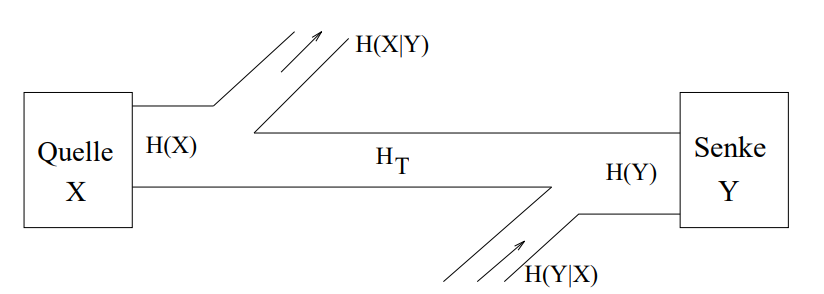
\includegraphics[scale=0.5]{./resources/berg_mod.png}
\end{figure}
\begin{itemize}
\item $H(X)$: Entropie Kanaleingang
\item $H(Y)$: Entropie Kanalausgang
\item $H_T$: Transinformation
\item $H(X\vert Y)$: Äquivokation (Rückschlussentropie)
\item $H(Y\vert X)$: Irrelevanz (Störentropie)
\end{itemize}
Note: Im Idealfall (ungestört) gilt $H(X) = H(Y) = H_T$

\paragraph{Transinformation\\}
Ist die im Mittel durch ein Kanalzeichen übertragene Informationsmenge
\begin{itemize}
\item $H_T = H(X) + H(Y) - H(X,Y) = H(X) - H(X \vert Y) = H(Y) - H(Y \vert X)$
\item Transinformation = Eingang minus 'Alles was verloren geht'
\item Transinformation = Ausgang minus 'Alles was dazu gekommen ist'
\end{itemize}

\subsection{Kanalkapazität}
Die Kanalkapazität C ist der Maximalwert des Transinformationsflusses $I_T$ ($\rightarrow C = max\{I_T \}$
\begin{figure}[H]
\centering
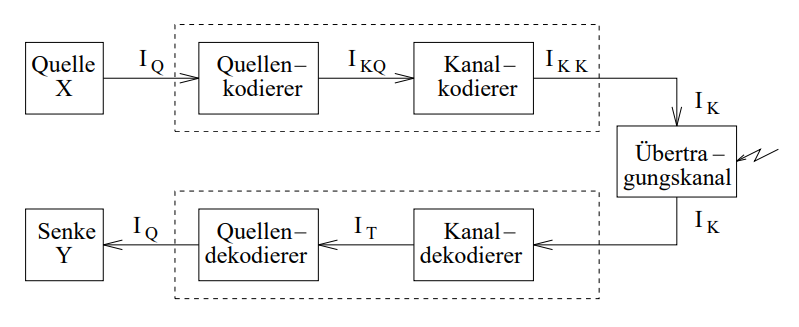
\includegraphics[scale=0.5]{./resources/kanal_cap.png}
\end{figure}
\begin{itemize}
\item $I_Q$: Quelleninformationsfluss ($I_Q =  f_Q H_Q$)
\item $I_{KQ}$: Quellenkodeinformationsfluss ($f_Q l H_K$ mit $l = \lceil \frac{ld\; N}{H_K}\rceil$)
\item $I_{KK}$: Kanalkodeinformationsfluss ($f_Q (l+\Delta l) H_K = f_Q n H_K$\\
mit Kanalkode $n= l + k, k \geq \rceil \Delta l \lceil)$)
\item $I_K$: Kanalinformationsfluss (= Übertragungsgeschwindigkeit $v_{"u}$) ($v_{"u} = I_K = v_s H_K$
\item $I_T$: Transinformationsfluss ($I_T = v_s H_T$)
\item $f_Q$: Quellensymbolfrequenz
\item $f_K$: Kanalsymbolfrequenz
\end{itemize}
Note: Der Transinformationsfluss $I_T$ eines gestörten Kanal ist immer kleiner als die Übertragungsgeschwindigkeit $v_{"u} = I_K$


\subsection{diskrete Binärkanal}
\begin{figure}[H]
\centering
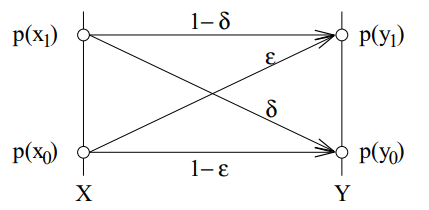
\includegraphics[scale=0.7]{./resources/gest_bk.png}
\end{figure}
\begin{itemize}
\item $\delta$: Wahrscheinlichkeit, dass das Zeichen $x_1$ in $y_0$ verfälscht wird
\item $\epsilon$: Wahrscheinlichkeit, dass das Zeichen $x_0$ in $y_1$ verfälscht wird
\item $1-\delta$, $1-\epsilon$: Wahrscheinlichkeit, dass das gesendete Zeichen richtig Übertragen wird
\item $(p(y_j\vert x_i)) = \begin{pmatrix}
1 - \epsilon & \epsilon\\
\delta & 1-\delta
\end{pmatrix}$
\end{itemize}

\paragraph{gesichert\\}
\begin{itemize}
\item $f_Q = \frac{v_{"u}}{n}$ ($v_{"u} = v_s$), ($n = l H_K^2$), ($n = \frac{H_K}{H_T}$)
\item $n = \frac{l}{H_T}$
\item $f_Q = \frac{v_{"u}H_t}{l}$
\end{itemize}

\paragraph{ungesichert\\}
\begin{itemize}
\item $v_s = f_q l$
\item $f_q = \frac{v_{"u}}{l}$
\end{itemize}

\paragraph{symmetrisch gestört\\}
$\epsilon = \delta = p_s$ (Die Wahrscheinlichkeit, dass ein Zeichen in ein anderes verfälscht wird, ist für alle Zeichen gleich
\begin{itemize}
\item $H_T = H(Y) - ((1-p_s)\, ld \, \frac{1}{(1-p_s)} + p_s \, ld \, \frac{1}{p_s})$
\item $H_{T_{max}} = 1 - ((1-p_s) \, ld \, \frac{1}{(1-p_s)} + p_s \, ld \, \frac{1}{p_s})$
\end{itemize}

\paragraph{einseitig gestört\\}
$\epsilon = p_s\; \delta = 0$  Nur ein Zeichen kann mit einer Wahrscheinlichkeit in ein anderes umgewandelt werden, das Andere wird immer sicher übertragen
\begin{itemize}
\item $H_T = H(Y) - p(x_0) \; ((1-p_s) \, ld \, \frac{1}{(1-p_s)} + p_s \, ld \, \frac{1}{p_s})$
\item $H_T = 1+\frac{1}{2} \, ((1+p_s) \, ld \, \frac{1}{(1+p_s)} - p_s \, ld \, \frac{1}{p_s})$
\end{itemize}
\newpage
\paragraph{Kanal mit Auslöschung\\}
Es wird ein Zusätzliches \textbf{Auslöschungszeichen} eingeführt mit Übergangswahrscheinlichkeit $\lambda$

\begin{itemize}
\item $H_{T_{max}} = (1-\lambda) - p_s \, ld \, \frac{1}{p_s} + (1-\lambda) \, ld \, \frac{1}{(1-\lambda)} - (1-p_s \lambda) \, ld \, \frac{1}{(1-p_s-\lambda)}$
\item Das Modell kann so umgeformt werden, dass Zeichen nicht in ein gültiges Kanalzeichen umgeformt werden können,\\
sondern nur in ein das Auslöschungszeichen (hier $y_2$)\\
$\rightarrow$ bessere Fehlerbehandlung
\item $H_{T_{max}} = (1-\lambda)$
\end{itemize}

\begin{figure}[H]
\begin{subfigure}{0.5\textwidth}
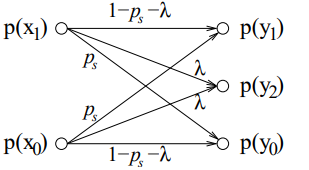
\includegraphics[scale=0.7]{./resources/bk_ausl.png}
\caption{Umwandlung in anderes Kodezeichen möglich}
\end{subfigure}
\begin{subfigure}{0.5\textwidth}
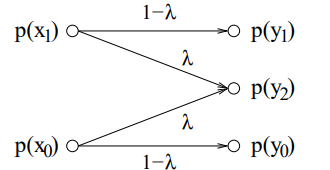
\includegraphics[scale=0.7]{resources/bk_ausl_2.png}
\caption{Umwandlung nur in Auslöschungzeichen möglich}
\end{subfigure}
\end{figure}


\subsection{analoge Kanäle}
Bei einem analogen Kanal ist es nicht möglich den Wert eines Zeichens klar zu bestimmen, vielmehr wird der Wert anhand einer Funktion beschrieben\\
Man kann dann die Wahrscheinlichkeit berechnen das der Wert sich in einem gewissen Intervall befindet\\
$p(x_i) = \int_{\Delta x} f(x) dx \approx f(x_i) \Delta x$
\begin{itemize}
\item $H_{diskr} = H_m \sum_i \, f(x_i) \, \Delta \, ld(\frac{1}{f(x_i)\Delta)}$
\item $H_{an} = \int_{-\infty}^{\infty} \, f(x) \, ld(\frac{1}{f(x)}) dx - ld \ \Delta x$
\item Da $ld \Delta x$ meist 0 nimmt man oft die \textbf{relative Entropie}\\
$H_{rel} = \int_{-\infty}^{\infty} \, f(x) \, ld(\frac{1}{f(x)}) dx$
\end{itemize}

\begin{figure}[H]
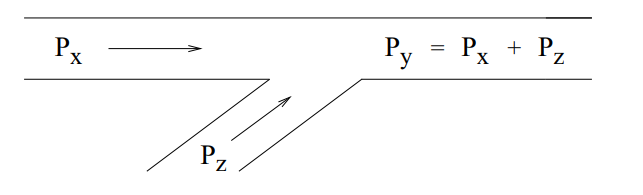
\includegraphics[scale=0.5]{./resources/ana_mod.png}
\end{figure}
\begin{itemize}
\item Signale und Störungen addieren sich $\rightarrow$ beide am Ausgang als Summe
\item keine Störsignale welche vom Nutzsignal abhängig sind\\
$\rightarrow$ Leistung des Empfangssignals ist die Summe aus Nutz- und Störsignalleistung
\end{itemize}

\paragraph{Transinformation\\}
\begin{itemize}
\item \textbf{Entropie}: $H(X) = \frac{1}{2} \, ld(2\pi \epsilon P_x)$
\item \textbf{Störentropie}: $H(Y\vert X) = \frac{1}{2} \, ld(2\pi \epsilon P_z)$
\item \textbf{Entropie Kanalausgang}: $H(Y) = \frac{1}{2} \, ld(2\pi \epsilon (P_x + P_z))$
\item \textbf{Transinformation}: $H_T = H(Y) - H(Y\vert X) = \frac{1}{2} \, ld(1 + \frac{P_x}{P_z})$ \\
wenn $\frac{P_x}{P_z} \gg 1$ dann $H_T \approx \frac{1}{2} \, ld \frac{P_x}{P_z}$
\item \textbf{Rauschabstand}: $r = 10 \, lg(\frac{P_x}{P_z})$
\item \textbf{Kanalkapazität}: $C_{an} = 2B\, H_T = 2B\frac{1}{2}(1+\frac{P_x}{P_z})$
\end{itemize}

\paragraph{Quantisierung\\}
\begin{itemize}
\item Zeitquantisierung
\begin{itemize}
\item $f_A \geq 2 f_g$
\item $t_A \leq \frac{1}{2 f_g} = \frac{1}{f_A}$\\
$\rightarrow$ bei Einhaltung kein Informationsverlust
\end{itemize}
\item Amplitudenquantisierung
\begin{itemize}
\item Informationsverlust
\end{itemize}
\end{itemize}



\section{Hamming-Code}

\subsection{Hamming-Distanz}
Die \textbf{Hamming Distanz} ($d(a_i, a_j)$) ist die Anzahl an Stellen um welche sich zwei Kodewörter unterscheiden. Für einen Binärkode gilt:\\
\begin{itemize}
\item \textbf{Hamming Distanz}: $d(a_i, a_j) = \sum_{g=1}^n \, (u_{ig} \oplus u_{jg})$ (Summe der XOR's aller Wörter)
\item \textbf{Mindestdistanz}: $d_{min} = \min_{a_i, a_j \in A, a_i \neq a_j} d(a_i, a_j)$
\item \textbf{Hamming Gewicht}: $w(a_i) = \sum_{g=1}^n \, u_{ig} = d(0, a_i)$
\end{itemize}

\paragraph{Fehlerkorrektur/erkennung\\}
Durch die Hamming Distanz können Fehler in den Kodewörten erkannt werden.\\
Indem Festgestellt wird, dass das erhaltene Kodewort nicht in der Gültigen Kodewortmenge liegt, kann erkannt werden, dass ein Fehler vorliegt ($f_e$). Liegt zudem das fehlerhafte Kodewort näher an einem anderen gültigen Kodewort (d.h. nicht exakt in der Mitte) so kann der Fehler sogar korrigiert werden ($f_k$)\\
Es gilt:
\begin{itemize}
\item $d_{min} = f_e + f_k + 1$
\item $f_e = \lfloor \frac{d_{min}}{2} \rfloor$
\item $f_k = \lfloor \frac{d_{min} - 1}{2} \rfloor$
\end{itemize}
\begin{figure}[H]
\centering
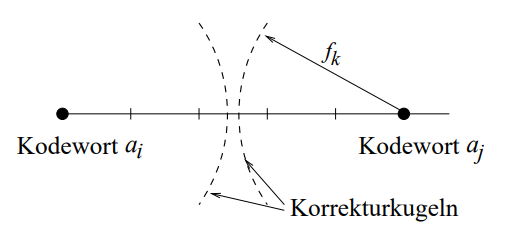
\includegraphics[scale=0.7]{./resources/kor_kug.png}
\end{figure}

\paragraph{Hamming-Schranke\\}
Anzahl der benötigten redundanten Stellen k
\begin{itemize}
\item $l = n - k$
\item $r_k = \frac{n-l}{n} = \frac{k}{n}$ (relative Redundanz)
\item $R = \frac{l}{n}$ (Koderate)
\end{itemize}
Ein Kode heißt \textbf{Perfekt} oder \textbf{dicht gepackt} wenn jedes Kodewort nur zu einem Wort einen geringsten Hammingabstand hat $\rightarrow$ jeder erkannte Fehler kann auch erkannt werden, da ein verfälschtes Kodewort immer einem Kodewort zugeordnet werden kann\\
$k \geq log_2(\sum_{i=0}^{f_k = 1}\binom{n}{i})$ mit $n = l + k $


\subsection{fehlerkorrigierender Hammingcode}
\begin{itemize}
\item $d_{min} =  3$, somit gilt auch $f_k = 1, f_e = 1$
\item $n = 2^k -1$
\end{itemize}


\paragraph{Kontrollmatrix}
\begin{figure}[H]
\centering
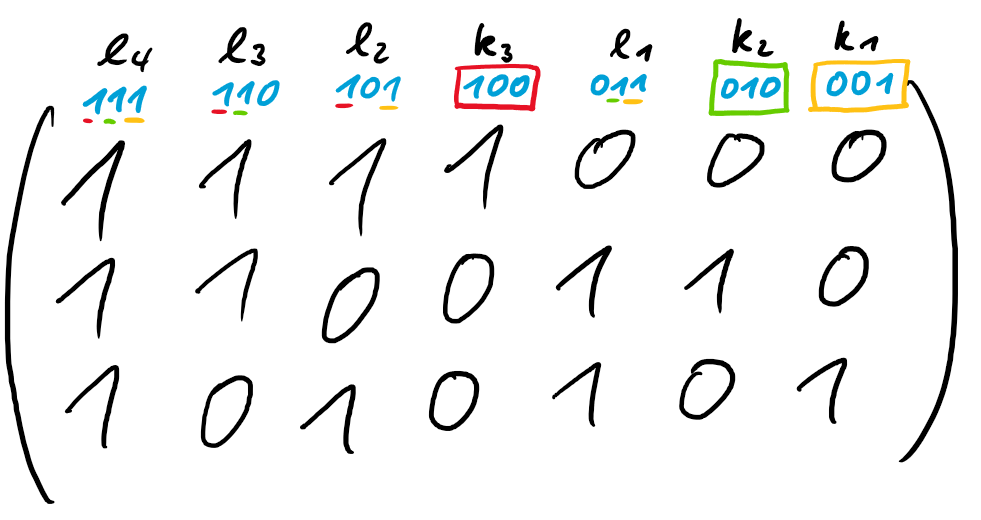
\includegraphics[scale=0.3]{./resources/hamming_control.png}
\caption{k... Kontrollstellen, l... Informationsstellen}
\end{figure}
\begin{itemize}
\item $k_3 = l_4 \oplus l_3 \oplus l_2$ (Stelle 3 := 1)
\item $k_2 = l_4 \oplus l_3 \oplus l_1$ (Stelle 2 := 1)
\item $k_1 = l_4 \oplus l_2 \oplus l_1$ (Stelle 1 := 1)
\end{itemize}

\paragraph{Fehlersyndrom}
How To machen:
\begin{enumerate}
\item Kontrollbit mit den dazugehörenden Informationsbits XORen
\item mach 1) für jede Zeile der Matrix
\item der dadurch erhaltene Vektor ist das Fehlersyndrom S
\begin{itemize}
\item S enthält nur Nullen $S = \vec{0}$ $\rightarrow$ kein Fehler gefunden
\item S enthält eine/mehrere Nullen $S \neq \vec{0}$ $\rightarrow$ ließ S als Zahl und flippe das Bit an dieser Stelle\\
z.B. $S = (1,0,0,1)$ $\rightarrow$ flippe Stelle 9
\end{itemize}
\end{enumerate}

\subsection{Erweiterter Hamming-Code}
\begin{itemize}
\item Fügt jedem Kanalkodewort ein weiteres Kontrollbit $k_0$ hinzu
\item $k_0$ wird dann hinten einfach angehangen
\item $n_0 = k_0 = \sum_i^n \, n_i mod 2$ (gerades Paritätsbit)
\item Erhöht $d_{min}$ auf 4 (von 3)
\end{itemize}


\section{Lineare Blockkodes (Linearkode)}
Ein Kode ist einer linear Blockkode wenn die Kodierungfunktion eine Verknüpfungsoperation einer Gruppe ist\\
Eigenschaften:
\begin{itemize}
\item Abgeschlossenheit
\item Assoziativität
\item neutrales Element
\item inverses Element
\item (kommutativ)* $\rightarrow$ abelsche Gruppe
\end{itemize}
Durch die obrigen Eigenschaften ergibt sich demnach auch:
\begin{itemize}
\item eine Verknüpfung eines Kanalkodewortes ergibt wieder ein Kanalkodewort (Abgeschlossenheit)
\item Nullwort ist immer ein Kanalkodewort (neutrales Element)
\item Fehlererkennung/korrektur:
\begin{itemize}
\item $f_e = d_{min} - 1$
\item $f_k = \lfloor \frac{d_{min} - 1}{2} \rfloor$, $f_e = \lfloor \frac{d_{min}}{2} \rfloor$ 
\end{itemize}
\end{itemize}

\paragraph{Systematischer Kode\\}
Ein Linearkode heißt systematisch, wenn man durch das Streichen der redundanten Stellen das Quellenwort erhält.\\
$\rightarrow$ z.B. Hamming Code durch streichen der Stellen $2^i$

\subsection{Generatormatrix}
How To machen:
\begin{enumerate}
\item jede Zeile von G muss ein Kodewort a sein
\item die Kodewörter müssen so ausgewählt werden das eine Einheitsmatrix der Größe l am Anfang entsteht ($I_n$)
\item Somit gilt dann $G_{l\times n} = [I_n C]$
\item Kodewörter können nun durch das Multiplizieren mit G kodiert werden\\
$a_i = a_i^* \cdot G$
\end{enumerate}

\subsection{Kontrollmatrix}
How To machen:
\begin{enumerate}
\item Sei C die Generatormatrix G ohne die Einheitsmatrix ($G_{l\times n} = [I_n C]$)
\item Transponiere C, dies bildet die ersten Spalten der Kontrollmatrix H
\item fülle den Rest (so das man auf n Spalten kommt) mit einer Einheitsmatrix ($I_K$) passender Größe auf
\item somit gilt dann: $H_{k, n} = [C^\top I_K]$
\item zum Prüfen eines Kodewortes multipliziere es mit der Kontrollmatrix\\
\begin{itemize}
\item Das Ergebnis ist gleich $\vec{0}$ $\rightarrow$ kein Fehler (oder zumindest keiner erkannt)
\item Das Ergebnis ist ungleich $\vec{0}$ $\rightarrow$ Fehler
\begin{itemize}
\item Das Ergebnis gleicht einer Spalte $n_i$ in H $\rightarrow$ flippe das Bit i
\item Das Ergebnis gleich keiner Spalte in H $\rightarrow$ nicht korrigierbar (Mehrfachfehler ?)
\end{itemize}
\end{itemize}
\end{enumerate}

\section{Zyklische Kodes}
Ein Kode in welchem durch zyklische Verschiebung der Elemente wieder ein Kanalkodewort entsteht\\
Ein zyklischer Kode ist ein spezieller Linearkode welcher Ring also auch Körperaxiome erfüllt\\
BCH-Codes können Bündelfehler $f_b$ erkennen mit $f_b \leq k$
\begin{itemize}
\item $m_1(x) = M(X)$
\item $m_0(x) = (x+1)$ (Abramson)
\end{itemize}

\subsection{Modularpolynome M(X)}
\begin{itemize}
\item \textbf{irreduzibel}: Ist nicht in ein Produkt von Polynomen zerlegbar\\
$M(X)$ bestimmt n mit $n \leq 2^{grad(M(X))} -1$
\item der tatsächliche Wert von n ergibt sich aus dem Zyklus der Polynomreste mit\\
$n = p \vert 2^{grad(M(X))} -1 $
\item \textbf{primitiv}: gilt $n=p=2^{grad(M(X))} - 1$ dann ist $M(X)$ auch primitiv\\
(es existiert eine Nullstelle $\alpha$ in $GF(p^m)$, so dass\\
$\{\alpha^n | \forall n \in \{0,...,p^m-2 \} \} = GF(p^m)$\\
Ein primitives Polynom ist wenn seine Nullstelle Ordnung $n = p^m - 1$ ist\\
ist $f(x)$ irreduzibel dann reicht $ggt(k,n) \neq 1$
\item Die Leistung des Kodes hängt von der Anzahl aufeinanderfolgender Nullstellen ab
\end{itemize}

\paragraph{Fundamentalsatz der Algebra\\}
Jedes Polynom r-ten Grades hat mindestens eine Nullstelle (ggf. in einem andern Körper) und lässt sich in genau r  Linearfaktoren zerteilen (mit Zuhilfenahme von Erweiterungselementen $\alpha_i$\\
Nimmt man nun eine Nullstelle $\alpha$ zu $M(X)$ hinzu entsteht ein endlicher Erweiterungskörper $GF(2^{k_1})$ mit Nullstelle $\alpha$ von $M(X)$ ($k_1 = grad(M(X))$)

\subsection{Generatorpolynom}
\begin{itemize}
\item Produkt von Minimalpolynom $m_i(x)$
\item beschreibt den Kode vollständig
\item $n = 2^{grad(M(x))} - 1 $ (da $M(X)$ primitiv)
\item $k = grad(g(x))$
\item $l = n-k$
\item $d_{min}$ tatsächlich aufeinanderfolgende Nullstellen + 1
\end{itemize}


% TODO
\subsection{Verfahren}
\subsubsection{Multiplikationsverfahren}
How To machen:
\begin{enumerate}
\item Multipliziere das Kodepolynom mit dem Generatorpolynom ($a(x) = a^*(x) g(x)$)
\end{enumerate}
\subsubsection{Divisionsverfahren}
How To machen:
\begin{enumerate}
\item Multipliziere das Kodepolynom mit $x^k$ ($k = grad(M)$)
\item Teile das Ergebnis mittel Polynomdivision über GF(2) und ermittle den Rest $r(x)$
\item Das Fertige Ergebnis ist nun $a(x) = a^*(x) \cdot x^k + r(x)$
\end{enumerate}

\paragraph{Fehlererkennung\\}
\begin{itemize}
\item $a(x) mod g(x) = 0$ kein Fehler
\item sonnst: Fehler
\end{itemize}

\paragraph{Kodes\\}
\begin{itemize}
\item Zyklischer Hamming Code: $d_{min} = 3$
\item Abramson Code: $d_{min} = 4$
\end{itemize}

\paragraph{Kodegeneration\\}
\begin{itemize}
\item Entwurfsabstand $d_E$ 
\item $g(x) = kgV\{m_{\mu}(x), ..., m_{\mu + d_E - 2}(x)\}$ mit $\mu \{0, 1\}$
\end{itemize}


\end{document}
